\section{Lecture 1}

\subsection{What is Computation?}

"Computation is the evolution process of some environment by a sequence of simple, local steps." 

\textcolor{blue}{- Avi Wigderson, \textit{Math \& Computation}}

Here are some examples of what computation may be:
\begin{itemize}
    \item How bits evolve in a computer.
    \item Computers in a network.
    \item Atoms in matter.
    \item Neurons in the brain.
    \item Prices in a market.
\end{itemize}

\begin{note} [Models of Computation]
    Mathematical modeling of computation gives us systematic ways to think and argue about computers.
    \begin{itemize}
        \item Independent of architecture.
        \item Idealized model: accurate in some aspects while not in others.
        \item Much simpler than an actual computer but captures key properties of it.
    \end{itemize}
\end{note}

Here is a roadmap.

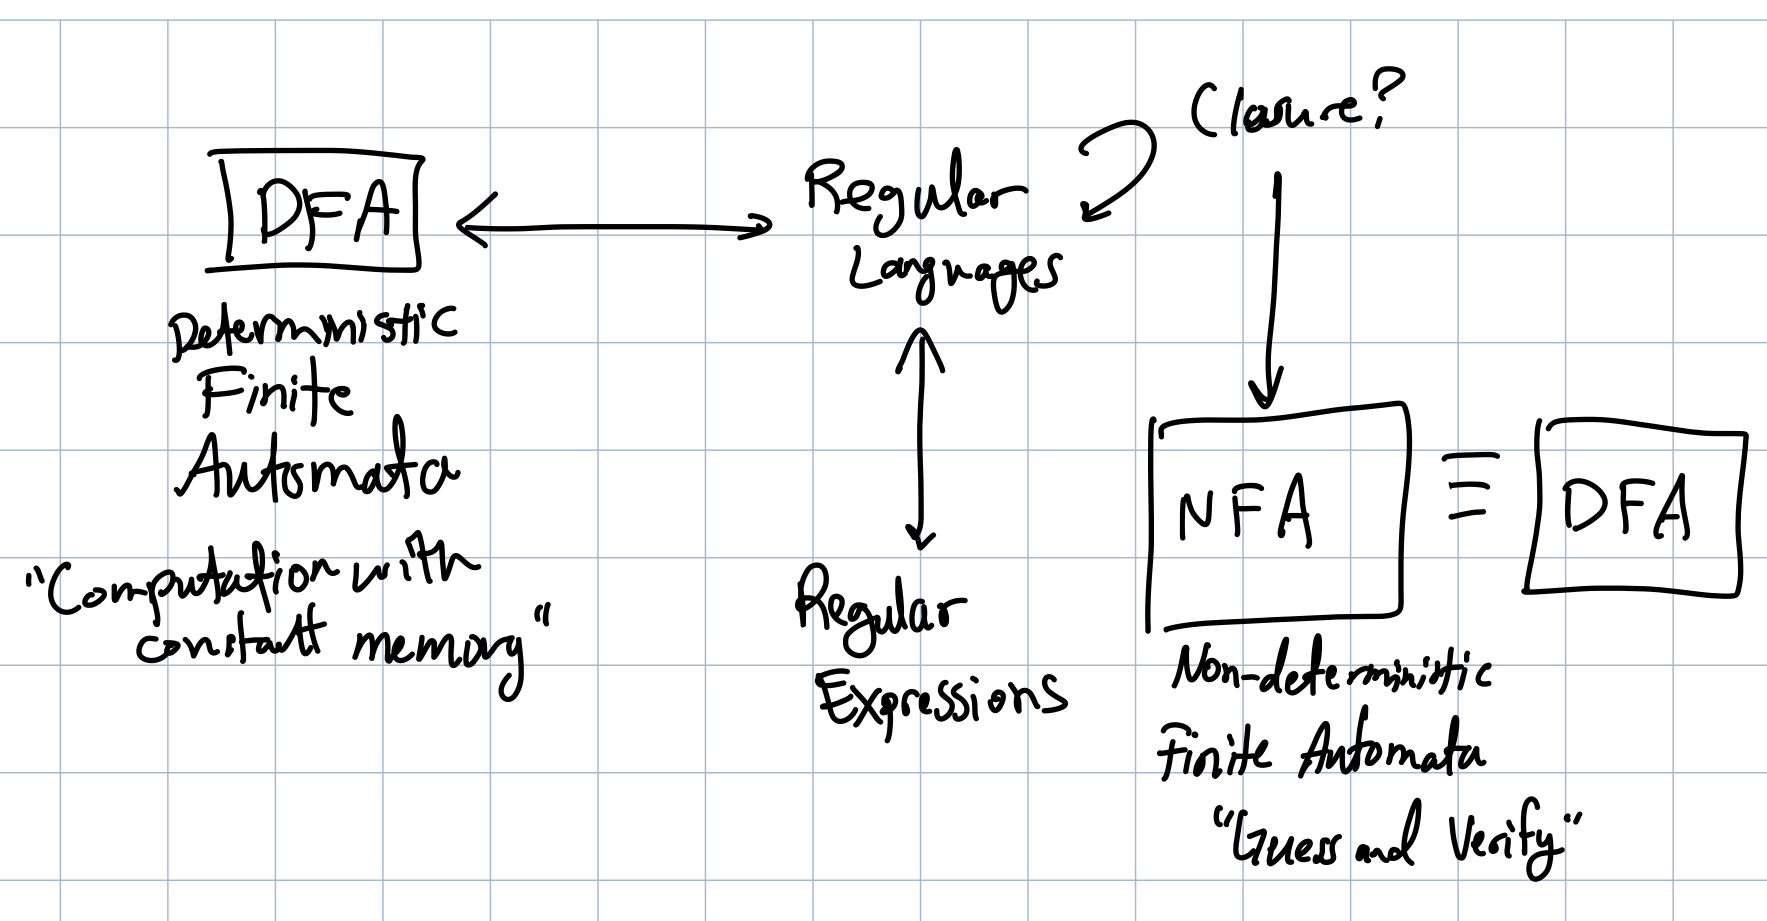
\includegraphics[width=300px]{roadmap.jpeg}

\subsection{Deterministic Finite Automata}

Here is a Deterministic Finite Automaton or Finite State Machine.

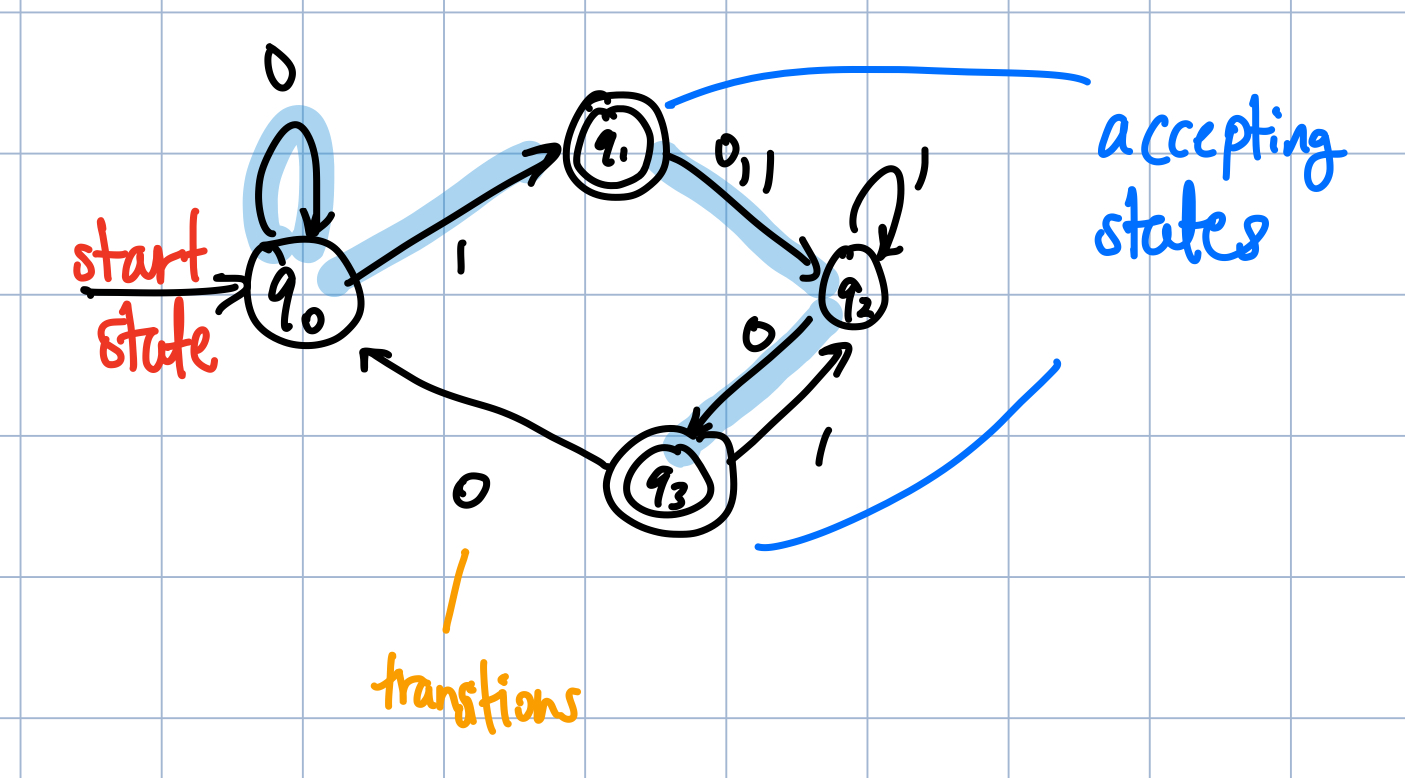
\includegraphics[width=300px]{dfa.jpeg}

A computation on 0110 is highlighted on the diagram. Since we ended at $q_3$, which is an accepting state. This means the string 0110 is accepted by this machine. A string that terminates a computation but it not accepted is rejected.

Why are DFAs useful?
\begin{itemize}
    \item They are a simple model of computation
    \item Useful for verification, compilers
    \item Close to Turing machines but we have a much better understanding of them
    \item Taste of "non-determinism", limitations
    \item Similar to streaming algorithms
\end{itemize}

\begin{definition}[Alphabet, String, Language]
    An alphabet $\Sigma$ is a finite set of characters, e.g. $\Sigma = \{0, 1\}$ or $\Sigma = \{A, \dots, Z\}$.

    A string over $\Sigma$ is a finite length sequence of symbols from $\Sigma$.

    For a string $x$, $|x|$ denotes the length of the string.

    In addition:
    \[ \Sigma^* = \{\text{string over $\Sigma$} \]
    And the empty string is $\varepsilon$, where $|\varepsilon| = 0$.

    A language over $\Sigma$ is a set of strings over $\Sigma$.
\end{definition}

Now we can formally define a DFA.

\begin{definition}[Deterministic Finite Automaton]
    A DFA (Deterministic Finite Automaton) is a 5-tuple $M = (Q, \Sigma, \delta, q_0, F)$:
    \begin{itemize}
        \item $Q$ is the set of all states
        \item $\Sigma$ is the alphabet
        \item $\delta: Q \times \Sigma \to Q$ is the transition function
        \item $q_0 \in Q$ is the start state
        \item $F \subseteq Q$ is the set of all accept/final states
    \end{itemize}
\end{definition}

Then we can define our computation more formally.

\begin{definition}[Computation Path, Acceptance]
    Let $w = w_1 w_2 \dots w_n$ be a string in $\Sigma^*$ of length $n$. The computation path of an automata $M$ on $w$ is the sequence of states
    $r_0, r_1, \dots, r_n \in Q$ defined by:
    \begin{itemize}
        \item $r_0 = q_0$
        \item $r_i = \delta(r_{i - 1}, w_i)$
    \end{itemize}
    $M$ accepts $w$ if and only if $r_n \in F$.
\end{definition}

And finally we get to the idea of a language corresponding to a DFA.

\begin{definition}
    If $M$ is a DFA, then $L(M)$, the language recognized by $M$ is the set of all strings that $M$ is accepted.
\end{definition}